% !TEX TS-program = knitr
\documentclass[handout]{beamer}\usepackage{graphicx, color}
%% maxwidth is the original width if it is less than linewidth
%% otherwise use linewidth (to make sure the graphics do not exceed the margin)
\makeatletter
\def\maxwidth{ %
  \ifdim\Gin@nat@width>\linewidth
    \linewidth
  \else
    \Gin@nat@width
  \fi
}
\makeatother

\IfFileExists{upquote.sty}{\usepackage{upquote}}{}
\definecolor{fgcolor}{rgb}{0.2, 0.2, 0.2}
\newcommand{\hlnumber}[1]{\textcolor[rgb]{0,0,0}{#1}}%
\newcommand{\hlfunctioncall}[1]{\textcolor[rgb]{0.501960784313725,0,0.329411764705882}{\textbf{#1}}}%
\newcommand{\hlstring}[1]{\textcolor[rgb]{0.6,0.6,1}{#1}}%
\newcommand{\hlkeyword}[1]{\textcolor[rgb]{0,0,0}{\textbf{#1}}}%
\newcommand{\hlargument}[1]{\textcolor[rgb]{0.690196078431373,0.250980392156863,0.0196078431372549}{#1}}%
\newcommand{\hlcomment}[1]{\textcolor[rgb]{0.180392156862745,0.6,0.341176470588235}{#1}}%
\newcommand{\hlroxygencomment}[1]{\textcolor[rgb]{0.43921568627451,0.47843137254902,0.701960784313725}{#1}}%
\newcommand{\hlformalargs}[1]{\textcolor[rgb]{0.690196078431373,0.250980392156863,0.0196078431372549}{#1}}%
\newcommand{\hleqformalargs}[1]{\textcolor[rgb]{0.690196078431373,0.250980392156863,0.0196078431372549}{#1}}%
\newcommand{\hlassignement}[1]{\textcolor[rgb]{0,0,0}{\textbf{#1}}}%
\newcommand{\hlpackage}[1]{\textcolor[rgb]{0.588235294117647,0.709803921568627,0.145098039215686}{#1}}%
\newcommand{\hlslot}[1]{\textit{#1}}%
\newcommand{\hlsymbol}[1]{\textcolor[rgb]{0,0,0}{#1}}%
\newcommand{\hlprompt}[1]{\textcolor[rgb]{0.2,0.2,0.2}{#1}}%

\usepackage{framed}
\makeatletter
\newenvironment{kframe}{%
 \def\at@end@of@kframe{}%
 \ifinner\ifhmode%
  \def\at@end@of@kframe{\end{minipage}}%
  \begin{minipage}{\columnwidth}%
 \fi\fi%
 \def\FrameCommand##1{\hskip\@totalleftmargin \hskip-\fboxsep
 \colorbox{shadecolor}{##1}\hskip-\fboxsep
     % There is no \\@totalrightmargin, so:
     \hskip-\linewidth \hskip-\@totalleftmargin \hskip\columnwidth}%
 \MakeFramed {\advance\hsize-\width
   \@totalleftmargin\z@ \linewidth\hsize
   \@setminipage}}%
 {\par\unskip\endMakeFramed%
 \at@end@of@kframe}
\makeatother

\definecolor{shadecolor}{rgb}{.97, .97, .97}
\definecolor{messagecolor}{rgb}{0, 0, 0}
\definecolor{warningcolor}{rgb}{1, 0, 1}
\definecolor{errorcolor}{rgb}{1, 0, 0}
\newenvironment{knitrout}{}{} % an empty environment to be redefined in TeX

\usepackage{alltt}
\newcommand{\answers}{1}

\setbeamercovered{dynamic}
\usetheme{Marburg}
\setbeamertemplate{navigation symbols}{} 
\setbeamertemplate{footline}
{
  \leavevmode%
  \hbox{%
  \begin{beamercolorbox}[wd=.333333\paperwidth,ht=2.25ex,dp=1ex,center]{author in head/foot}%
    \usebeamerfont{author in head/foot}\copyright $\ $ \insertshortauthor%~~\beamer@ifempty{\insertshortinstitute}{}{(\insertshortinstitute)}
  \end{beamercolorbox}%
  \begin{beamercolorbox}[wd=.333333\paperwidth,ht=2.25ex,dp=1ex,center]{title in head/foot}%
    \usebeamerfont{title in head/foot} \insertinstitute
  \end{beamercolorbox}%
  \begin{beamercolorbox}[wd=.333333\paperwidth,ht=2.25ex,dp=1ex,right]{date in head/foot}%
    \usebeamerfont{date in head/foot}\insertshortdate{}\hspace*{2em}
    \insertframenumber{} / \inserttotalframenumber\hspace*{2ex} 
  \end{beamercolorbox}}%
  \vskip0pt%
}

\usepackage{amsmath}
\usepackage{caption}
\usepackage{color}
\usepackage{enumerate}
\usepackage{listings}
\usepackage{hyperref}
\usepackage{mathrsfs}
\usepackage{natbib}
\usepackage{url}

\providecommand{\all}{\ \forall \ }
\providecommand{\bs}{\backslash}
\providecommand{\e}{\varepsilon}
\providecommand{\E}{\ \exists \ }
\providecommand{\lm}[2]{\lim_{#1 \rightarrow #2}}
\providecommand{\m}[1]{\mathbb{#1}}
\providecommand{\nv}{{}^{-1}}
\providecommand{\ov}[1]{\overline{#1}}
\providecommand{\p}{\newpage}
\providecommand{\q}{$\quad$ \newline}
\providecommand{\rt}{\rightarrow}
\providecommand{\Rt}{\Rightarrow}
\providecommand{\vc}[1]{\boldsymbol{#1}}
\providecommand{\wh}[1]{\widehat{#1}}

\hypersetup{colorlinks,linkcolor=,urlcolor=blue}
\numberwithin{equation}{section}

\definecolor{dkgreen}{rgb}{0,0.6,0}
\definecolor{gray}{rgb}{0.5,0.5,0.5}
\definecolor{mauve}{rgb}{0.58,0,0.82}

\lstset{ 
  language=C,                % the language of the code
  basicstyle= \footnotesize,           % the size of the fonts that are used for the code
  numberstyle= \tiny \color{white},  % the style that is used for the line-numbers
  stepnumber=2,                   % the step between two line-numbers. 
  numbersep=5pt,                  % how far the line-numbers are from the code
  backgroundcolor=\color{white},      % choose the background color. You must add \usepackage{color}
  showspaces=false,               % show spaces adding particular underscores
  showstringspaces=false,         % underline spaces within strings
  showtabs=false,                 % show tabs within strings adding particular underscores
  frame=lrb,                   % adds a frame around the code
  rulecolor=\color{black},        % if not set, the frame-color may be changed on line-breaks within not-black text 
  tabsize=2,                      % sets default tabsize to 2 spaces
  captionpos=t,                   % sets the caption-position 
  breaklines=true,                % sets automatic line breaking
  breakatwhitespace=false,        % sets if automatic breaks should only happen at whitespace
  %title=\lstname,                   % show the filename of files included with \lstinputlisting;
  keywordstyle=\color{blue},          % keyword style
  commentstyle=\color{gray},       % comment style
  stringstyle=\color{dkgreen},         % string literal style
  escapeinside={\%*}{*)},            % if you want to add LaTeX within your code
  morekeywords={*, ...},               % if you want to add more keywords to the set
  xleftmargin=0.053in, % left horizontal offset of caption box
  xrightmargin=-.03in % right horizontal offset of caption box
}

%\DeclareCaptionFont{white}{\color{white}}
%\DeclareCaptionFormat{listing}{\parbox{\textwidth}{\colorbox{gray}{\parbox{\textwidth}{#1#2#3}}\vskip-0.05in}}
%\captionsetup[lstlisting]{format = listing, labelfont = white, textfont = white}
%For caption-free listings, comment out the 3 lines above and uncomment the 2 lines below.
 \captionsetup{labelformat = empty, labelsep = none}
 \lstset{frame = single}




\title{Discrete Random Variables (Ch. 5.1)}
\author{Will Landau}
\date{Feb 7, 2013}
\institute{Iowa State University}

\begin{document}

\begin{frame}
\titlepage
 \end{frame}
 
 \AtBeginSection[]
{
   \begin{frame}
       \frametitle{Outline}
       \tableofcontents[currentsection]
   \end{frame}
}

\section{What is a random variable?}

\begin{frame}
\frametitle{What is a random variable?}
\begin{itemize}
\pause \item {\bf Random variable}; a quantity that can be thought of as dependent on chance phenomena.
\begin{itemize}
\pause \item $X = $ the value of a coin toss (heads or tails).
\pause \item $Z = $ the amount of torque required to loosen the next bolt.
\pause \item $T = $ the time you'll have to wait for the next bus home.
\pause \item $N = $ the number of defective widgets in manufacturing process in a day.
\pause \item $S = $ the number of provoked shark attacks off the coast of Florida next year.
\end{itemize}
\pause \item Two types:
\begin{itemize}
\pause \item {\bf Discrete random variable}: one that can only take on a set of isolated points ($X$, $N$, and $S$).
\pause \item {\bf Continuous random variable}: one that can fall in an interval of real numbers ($T$ and $Z$). 
\end{itemize}
\end{itemize}
\end{frame}

\begin{frame}
\frametitle{Discrete random variables}
\begin{itemize}
\pause \item A discrete random variable has a list of possible values:
\begin{itemize}
\pause \item $X = $ roll of a 6-sided fair die = 1, 2, 3, 4, 5, or 6.
\pause \item $Y = $ roll of a 6-sided \emph{unfair} die = 1, 2, 3, 4, 5, or 6. 
\end{itemize}
\pause \item But how do you distinguish between $X$ and $Y$?
\end{itemize}
\end{frame}

\section{Probability}

\begin{frame}
\frametitle{Probability}
\begin{itemize}
\pause \item $P(X = x)$, the {\bf probability} that $X$ equals $x$, is the fraction of times that $X$ will land on $x$
\begin{enumerate}[1. ]
\pause \item We expect a fair die to land the number 3 roughly one out of every 6 tosses. Thus, $P(X = 3) = 1/6$
\pause \item Suppose the unfair die is weighted so that the number 3 only lands one out of every 22 tosses. Then, $P(Y = 3) = 1/22$. 
\end{enumerate}
\end{itemize}
\end{frame}


\begin{frame}

\begin{itemize}
\item $X$ has the following probabilities: \q 
\end{itemize}
\begin{tabular}{ccccccc}
$x$ & 1 & 2 & 3 & 4 & 5 & 6 \\ \hline
$P(X = x)$ & 1/6 & 1/6 & 1/6 & 1/6 & 1/6 & 1/6 
\end{tabular} 

\begin{center}
\begin{knitrout}
\definecolor{shadecolor}{rgb}{0.969, 0.969, 0.969}\color{fgcolor}
\includegraphics[width=.6\textwidth,height=.6\textheight]{figure/unnamed-chunk-2} 

\end{knitrout}

\end{center}


\end{frame}

\begin{frame}
\begin{itemize}
\item Say $Y$ has the probabilities: \q 
\end{itemize}
\begin{tabular}{ccccccc}
$y$ & 1 & 2 & 3 & 4 & 5 & 6 \\ \hline
$P(Y = y)$ & 5/22 & 7/44 & 1/22 & 7/44 & 2/11 & 5/22
\end{tabular} 

\begin{center}
\begin{knitrout}
\definecolor{shadecolor}{rgb}{0.969, 0.969, 0.969}\color{fgcolor}
\includegraphics[width=.6\textwidth,height=.6\textheight]{figure/unnamed-chunk-3} 

\end{knitrout}

\end{center}

\end{frame}

\begin{frame}
\begin{itemize}
\item $S$, the number of provoked shark attacks off FL next year, has infinite number of possible values. Here is one possible (made up) distribution: \q \q
\end{itemize}
\begin{tabular}{ccccccc}
$s$ & 1 & 2 & 3 & $\cdots$ & $k$ & $\cdots$ \\ \hline
$P(S = s)$ & $\frac{6}{\pi^2}$ & $\frac{1}{2} \frac{6}{\pi^2}$ & $\frac{1}{4} \frac{6}{\pi^2}$ & $\cdots$ & $\frac{1}{2^k} \frac{6}{\pi^2}$ & $\cdots$ \\ 
\end{tabular}\q

\begin{center}
\begin{knitrout}
\definecolor{shadecolor}{rgb}{0.969, 0.969, 0.969}\color{fgcolor}
\includegraphics[width=.6\textwidth,height=.6\textheight]{figure/unnamed-chunk-4} 

\end{knitrout}

\end{center}
\begin{itemize}
\item \emph{But all the probabilities for a random variable have to add up to 1.}
\end{itemize}
\end{frame}

\section{Probability Mass Functions (pmf)}

\begin{frame}
\frametitle{Probability mass functions (pmf)}
\begin{itemize}
\pause \item The {\bf probability mass function (pmf)} $f(x)$ of a random variable $X$ is just $P(X = x)$
\begin{itemize}
\pause \item $X$ has $f(x) = 1/6$
\pause \item $S$ has $f(s) = \frac{1}{2^s} \frac{6}{\pi^2}$.
\end{itemize}
\pause \item We could also write $f_X$ for the pmf of $X$ and $f_S$ for the pmf of $S$. 
\pause \item \color{blue} Rules of the pmf $f$:
\begin{itemize}
\pause \item \color{blue} $f(x) \ge 0$ for all $x$.
\pause \item \color{blue} $\sum_x f(x) = 1$. 
\end{itemize}
\end{itemize}
\color{black}
\end{frame}


\begin{frame}
\frametitle{Your turn: calculating probabilities} \scriptsize
\begin{itemize}
\item Let $Z$ = the torque, rounded to the nearest integer, required to loosen the next bolt on an apparatus. \q 


\begin{center}
\begin{tabular}{ccccccccccc}
$z$ & 11 & 12 & 13 & 14 & 15 \\ \hline
$f(z) = P(Z = z)$ & 0.03 & 0.03 & 0.03 & 0.06 & 0.26 
\end{tabular} \q

\begin{tabular}{ccccccccccc}
$z$ & 16 & 17 & 18 & 19 & 20 \\ \hline
$f(z) = P(Z = z)$ &  0.09 & 0.12 & 0.20 & 0.15 & 0.03 
\end{tabular} \q \q

\begin{knitrout}
\definecolor{shadecolor}{rgb}{0.969, 0.969, 0.969}\color{fgcolor}
\includegraphics[width=.4\textwidth,height=.3\textheight]{figure/unnamed-chunk-5} 

\end{knitrout}

\end{center}
\item Calculate:
\begin{enumerate}[1. ]
\item $P(Z \le 14)$
\item $P(Z > 16)$
\item $P(Z \text{ is an even number})$
\item $P(Z \text{ in } \{15, 16, 18\})$
\end{enumerate}
\end{itemize}
\end{frame}

\begin{frame}<handout:\answers>
\frametitle{Answers: calculating probabilities} \scriptsize
\begin{enumerate}[1. ]
\item \begin{align*}
\uncover<1->{P(Z \le 14)} & \uncover<1->{= P(Z = 11 \text{ or } Z = 12 \text{ or } Z = 13 \text{ or } Z = 14)} \\
& \uncover<2->{= P(Z = 11) + P(Z = 12) + P(Z = 13) + P(Z = 14)} \\
& \uncover<3->{= f(11) + f(12) + f(13) + f(14)} \\
& \uncover<4->{= 0.03 + 0.03 + 0.03 + 0.06} \\
& \uncover<5->{= 0.15 }
\end{align*}
\item 
\begin{align*}
\uncover<6->{P(Z > 16)} & \uncover<6->{= P(Z = 17 \text{ or } Z = 18 \text{ or } Z = 19 \text{ or } Z = 20)} \\
&\uncover<7->{ = P(Z = 17) + P(Z = 18) + P(Z = 19) + P(Z =20)} \\
& \uncover<8->{= f(17) + f(18) + f(19) + f(20)} \\
& \uncover<9->{= 0.12 + 0.20 + 0.15 + 0.03} \\
& \uncover<10->{= 0.5}
\end{align*}
\end{enumerate}
\end{frame}

\begin{frame}<handout:\answers>
\frametitle{Answers: calculating probabilities} \scriptsize
\begin{enumerate}
\setcounter{enumi}{2}
\item 
\begin{align*}
\uncover<1->{P(Z \text{ even})} & \uncover<1->{= P(Z = 12 \text{ or } Z = 14 \text{ or } Z = 16 \text{ or } Z = 18 \text{ or } Z = 20)} \\
& \uncover<2->{=  P(Z = 12) +  P(Z = 14) +  P(Z = 16) +  P(Z = 18)} \\
 & \uncover<2->{\quad +   P(Z = 20)} \\
&\uncover<3->{ = f(12) + f(14) + f(16) + f(18) + f(20)} \\
& \uncover<4->{= 0.03 + 0.06 + 0.09 + 0.20 + 0.03} \\
& \uncover<5->{= 0.41}
\end{align*}

\item 
\begin{align*}
\uncover<6->{P(Z \text{ in } \{15, 16, 18\})} & \uncover<6->{= P(Z = 15 \text{ or } Z = 16 \text{ or } Z = 18)} \\
&\uncover<7->{ = P(Z = 15) + P(Z = 16) + P(Z = 18)} \\
&\uncover<8->{ = f(15) + f(16) + f(18)} \\
&\uncover<9->{ = 0.26 + 0.09 + 0.02 }\\
&\uncover<10->{ = 0.37}
\end{align*}
\end{enumerate}
\end{frame}










\section{Cumulative Distribution Functions (cdf)}

\begin{frame}
\frametitle{The cumulative distribution function (cdf)}

\begin{itemize}
\item {\bf Cumulative distribution function (cdf)}: a function, $F$, defined by:
\begin{align*}
\uncover<2->{F(x)} &\uncover<2->{= P(X \le x)}\\
& \uncover<3->{= \sum_{z \le x} f(z)}
\end{align*}
\pause \pause  \pause \item $F$ has the following properties:
\begin{itemize}
\pause \item $F(x) \ge 0$ for all real numbers $x$.
\pause \item $F$ is monotonically increasing.
\pause \item $\lim_{x \rt -\infty} F(x) = 0$
\pause \item $\lim_{x \rt \infty} F(x) = 1$
\end{itemize}
\pause \item When statisticians say ``distribution", they mean cdf.
\end{itemize}
\end{frame}

\begin{frame}
\frametitle{Example: torque random variable, $Z$}
\setkeys{Gin}{width=1\textwidth} 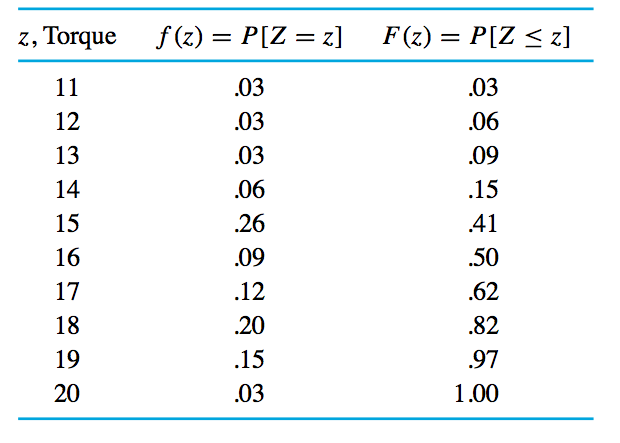
\includegraphics{../../fig/torquep.png}
\end{frame}


\begin{frame}
\frametitle{Example: torque random variable, $Z$}
\setkeys{Gin}{width=1\textwidth} 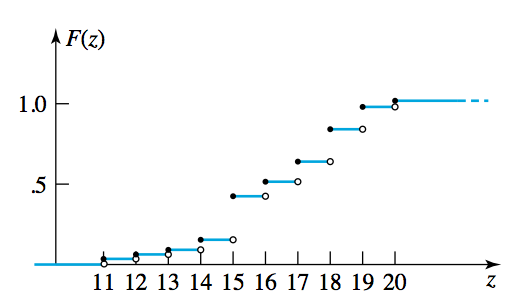
\includegraphics{../../fig/torquez.png}
\end{frame}


\begin{frame}
\frametitle{Your turn: calculating probabilities} \scriptsize

\begin{center}
\begin{tabular}{ccccccccccc}
$z$ & 11 & 12 & 13 & 14 & 15 \\ \hline
$F(z) = P(Z \le z)$ & 0.03 & 0.06 & 0.09 & 0.15 & 0.41
\end{tabular} \q

\begin{tabular}{ccccccccccc}
$z$ & 16 & 17 & 18 & 19 & 20 \\ \hline
$F(z) = P(Z \le z)$ &  0.50 & 0.62 & 0.82 & 0.97 & 1 
\end{tabular} \q 
\setkeys{Gin}{width=.5\textwidth} 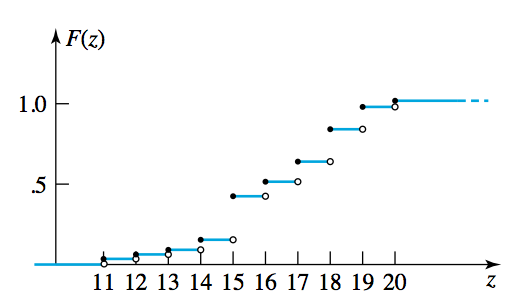
\includegraphics{../../fig/torquez.png}
\end{center}

\begin{itemize}
\item Using the cdf only, calculate:
\begin{enumerate}[1. ]
\item F(10.7)
\item $P(Z \le 15.5)$
\item $P( 12.1 < Z \le 14)$
\item $P( 15 \le Z <  18)$
\end{enumerate}
\end{itemize}
\end{frame}








\begin{frame}<handout:\answers>
\frametitle{Answers: calculating probabilities}
\begin{enumerate}[1. ]
\pause \item $F(10.7) = P(Z \le 10.7) = 0$
\pause \item $P(Z \le 15.5) = P(Z \le 15)  = 0.41$
\pause \item \begin{align*}
\uncover<4->{P( 12.1 < Z \le 14)} & \uncover<4->{= P(Z = \text{13 or 14})} \\
& \uncover<5->{ = f(14) + f(13)} \\
& \uncover<6->{ = [f(14) + f(13) + f(12) + f(11)] } \\
& \uncover<6->{\quad - [f(12) + f(11)]} \\
& \uncover<7->{= P(Z \le 14) - P(Z \le 12)} \\
& \uncover<8->{ = F(14) - F(12)} \\
& \uncover<9->{= 0.15 - 0.06} \\
& \uncover<10->{= 0.09}
\end{align*}
\end{enumerate}
\end{frame}

\begin{frame}<handout:\answers>
\frametitle{Answers: calculating probabilities}
\begin{enumerate}
\setcounter{enumi}{3}
\item 
\begin{align*}
\uncover<1->{P(15 \le Z <  18)} & \uncover<1->{= P(Z = \text{15, 16, or 17})} \\
& \uncover<2->{= P(Z \le 17) - P(Z \le 14)} \\
& \uncover<3->{= F(17) - F(14)} \\
& \uncover<4->{= 0.62 - 0.15} \\
& \uncover<5->{= 0.47}
\end{align*}
\end{enumerate}
\end{frame}


\begin{frame}
\frametitle{Your turn: drawing the cdf}

\begin{itemize}
\item Say we have a random variable $Q$ with pmf: \q \q
\begin{tabular}{ccccc}
$q$ & 1 & 2 & 3 & 7  \\ \hline
$f(q)$ & 0.34 & 0.1 & 0.22 & 0.34\\
\end{tabular} \q
\item Draw the cdf.
\end{itemize}
\end{frame}


\begin{frame}<handout:\answers>
\frametitle{Answer: drawing the cdf}

\begin{knitrout}
\definecolor{shadecolor}{rgb}{0.969, 0.969, 0.969}\color{fgcolor}
\includegraphics[width=0.8\textwidth,height=0.8\textheight]{figure/unnamed-chunk-6} 

\end{knitrout}

\end{frame}

\section{Expected Value}


\begin{frame}
\frametitle{Expected Value} \small
\begin{itemize}
\pause \item The {\bf expected value} $E(X)$ (also called $\mu$) of a random variable $X$ is given by:
\begin{align*}
\sum_{x} x \cdot f(x)
\end{align*}
\pause \item When $X$ is the roll of a fair die,
\begin{align*}
\uncover<4->{E(X)} & \uncover<4->{= 1 f(1) + 2 f(2) + 3 f(3) + 4 f(4) + 5 f(5) + 6 f(6)} \\
& \uncover<5->{= 1 (1/6) + 2 (1/6) + 3 (1/6) + 4 (1/6) + 5 (1/6) + 6 (1/6)} \\ 
& \uncover<6->{= \frac{1+2+3+4+5+6}{6}} \\
& \uncover<7->{= 3.5}
\end{align*}
\pause \pause \pause \pause \pause \item $E(X)$ is a \emph{weighted average} of the possible values of $X$, weighted by their probabilities.
\pause \item $E(X)$ is the {\bf mean of the distribution} of $X$
\end{itemize}
\end{frame}




\begin{frame}
\frametitle{Your turn: expected value}

\begin{tabular}{ccccccc}
$y$ & 1 & 2 & 3 & 4 & 5 & 6 \\ \hline
$P(Y = y)$ & 5/22 & 7/44 & 1/22 & 7/44 & 2/11 & 5/22
\end{tabular} 

\begin{center}
\begin{knitrout}
\definecolor{shadecolor}{rgb}{0.969, 0.969, 0.969}\color{fgcolor}
\includegraphics[width=.6\textwidth,height=.6\textheight]{figure/unnamed-chunk-7} 

\end{knitrout}

\end{center}

\begin{itemize}
\item Calculate $E(Y)$, the expected value of a toss of the \emph{unfair} die.
\end{itemize}
\end{frame}




\begin{frame}<handout:\answers>
\frametitle{Answer: expected value}\scriptsize
\begin{itemize}
\item 
\begin{align*}
\uncover<1->{E(Y)} & \uncover<1->{= 1 (5/22) + 2(7/44) + 3 (1/22)} \\
&\uncover<1->{ \qquad + 4(7/44) + 5(2/11) + 6(5/22)} \\
&\uncover<2->{ = 3.5909}
\end{align*}
\pause \pause \item The average roll of the unfair die is 3.5909.
\pause \item $E(Y)$ is the  mean of the distribution of $Y$.
\end{itemize}

\begin{center}
\begin{knitrout}
\definecolor{shadecolor}{rgb}{0.969, 0.969, 0.969}\color{fgcolor}
\includegraphics[width=.4\textwidth,height=.4\textheight]{figure/unnamed-chunk-8} 

\end{knitrout}

\end{center}
\end{frame}



\begin{frame}
\frametitle{Your turn: expected value}

\begin{center}
\begin{tabular}{ccccccccccc}
$z$ & 11 & 12 & 13 & 14 & 15 \\ \hline
$f(z) = P(Z = z)$ & 0.03 & 0.03 & 0.03 & 0.06 & 0.26 
\end{tabular} \q

\begin{tabular}{ccccccccccc}
$z$ & 16 & 17 & 18 & 19 & 20 \\ \hline
$f(z) = P(Z = z)$ &  0.09 & 0.12 & 0.20 & 0.15 & 0.03 
\end{tabular} \q 
\end{center}

\begin{itemize}
\item Calculate $E(Z)$, the expected value of the torque required to loosen the next bolt.
\end{itemize}
\end{frame}

\begin{frame}<handout:\answers>
\frametitle{Answer: expected value}\scriptsize
\begin{align*}
\uncover<1->{E(Z)} & \uncover<1->{= 11 (0.03) + 12(0.03) + 13(0.03) + 14(0.06) + 15(0.26)} \\
& \uncover<2->{= 16(0.09) + 17(0.12) + 18(0.20) + 19(0.15) + 20(0.03)} \\
& \uncover<3->{= 16.35}
\end{align*}

\begin{itemize}
\pause \pause \pause \item The average torque required to loosen the next bolt is 16.35 units.
\end{itemize}
\end{frame}






\section{Variance and Standard Deviation}

\begin{frame}
\frametitle{Variance}
\begin{itemize}
\pause \item {\bf Variance}: the variance $Var(X)$ (also called $\sigma^2$) of a random variable $X$ is given by:
\begin{align*}
\text{Var} (X) &= \sum_x (x - E(X))^2 f(x) \\
\end{align*}
\pause \item Shortcut formulas:
\begin{align*}
\uncover<3->{\text{Var} (X) }  & \uncover<3->{= \left [ \sum_x x^2 f(x) \right ]  - (E(X))^2} \\
 & \uncover<4->{= E(X^2) - E^2(X)} \\
\end{align*}
\pause \pause \item The variance is the average squared deviation of random variable from its mean.
\pause \item {\bf Standard deviation}: $SD(X) = \sigma = \sqrt{Var(X)}$
\end{itemize}
\end{frame}

\begin{frame}
\frametitle{Example: calculating the variance} \scriptsize
\begin{tabular}{ccccc}
$q$ & 1 & 2 & 3 & 7  \\ \hline
$f(q)$ & 0.34 & 0.1 & 0.22 & 0.34\\
\end{tabular} \q

\begin{itemize}
\item Long way:
\begin{align*}
\uncover<1->{E(Q)} &= \uncover<1->{ 1 (0.34) + 2(0.1) + 3(0.22) + 7(0.34) }\\
& \uncover<2->{= 3.58} \\
\uncover<3->{Var (Q)} & \uncover<3->{= (1 - 3.58)^2 0.34 + (2-3.58)^2 0.1} \\
& \uncover<3->{\qquad + (3 - 3.58)^2 0.22 + (7-3.58)^2 0.34} \\
& \uncover<4->{= 6.56}
\end{align*}
\uncover<5->{\item Short way:}


\begin{align*}
\uncover<5->{E(Q^2)} & \uncover<5->{= \sum_{q} q^2 f(q)} \\
&\uncover<6->{ = 1 (0.34) + 4(0.1) + 9(0.22) + 49(0.34)} \\
& \uncover<7->{= 19.38} \\
\uncover<8->{Var(Q) }& \uncover<8->{= E(Q^2) - E^2(Q)} \\
& \uncover<9->{= 19.38 - 3.58^2} \\
&\uncover<10->{ = 6.56}
\end{align*}
\end{itemize}
\end{frame}


\begin{frame}
\frametitle{Your turn: calculating the variance}

\begin{tabular}{ccccccc}
$x$ & 1 & 2 & 3 & 4 & 5 & 6 \\ \hline
$f(x)$ & 1/6  & 1/6  & 1/6  & 1/6  & 1/6  & 1/6  \\
\end{tabular}

\begin{itemize}
\item Calculate $Var(X)$
\item Calculate $SD(X)$
\end{itemize}
\end{frame}


\begin{frame}<handout:\answers>
\frametitle{Your turn: answers} \scriptsize

\begin{itemize}
\item
\begin{align*}
\uncover<1->{E(X)} &\uncover<1->{= 1 (1/6) + 2(1/6) + 3(1/6) + 4(1/6) + 5(1/6) + 6 (1/6)} \\
&\uncover<2->{ = 3.5} \\
\uncover<3->{E(X^2)} & \uncover<3->{= \sum_{x = 1}^6 x^2 f(x)} \\
&\uncover<4->{ = 1^2 (1/6) + 2^2(1/6) + 3^2(1/6) + 4^2(1/6) + 5^2(1/6) + 6 ^2(1/6)}  \\
& \uncover<5->{=  15.17} \\
\uncover<5->{Var(X)} &\uncover<5->{ = E(X^2) - E^2(X)} \\
& \uncover<6->{= 15.17 - 3.5^2} \\
&\uncover<7->{ = 2.92}
\end{align*}
\item \uncover<8->{$SD(X) = \sqrt{2.92} = 1.7088$}
\end{itemize}
\end{frame}

\end{document}
